\section{生物能学}

\section{生物氧化}

\begin{table}[htbp]
	\centering
	\begin{tabularx}{\textwidth}{|c|c|C|}
		\hline
		抑制类型 & 抑制剂名称 & 作用位点或作用机制 \\ \hline
		\multirow{4}{*}{呼吸链抑制剂} & 鱼藤酮、安米妥、杀粉菌素 & 复合体 I \\ \cline{2-3}
		& 萎锈灵 & 复合体 II \\ \cline{2-3}
		& 抗霉素 A & 复合体 III \\ \cline{2-3}
		& 氰化物、CO、H₂S、叠氮化物 & 复合体 IV \\ \hline
		\multirow{3}{*}{F₁F₀-ATP 合酶抑制剂} & 金轮霉素 & 抑制 F₁ \\ \cline{2-3}
		& 寡霉素、杀黑星菌素 & 抑制 F₀ \\ \cline{2-3}
		& DCCD & 阻止质子通过 F₀ 通道 \\ \hline
		\multirow{3}{*}{解偶联剂} & DNP、FCCP & 脂溶性质子载体 \\ \cline{2-3}
		& 缬氨霉素 & 钾离子载体,破坏电势能 \\ \cline{2-3}
		& 生热素 & 质子通道 \\ \hline
		ATP/ADP 交换体抑制剂 & 苍术苷、米酵菌酸 & 抑制线粒体基质内的 ATP 与细胞质内的 ADP 之间交换 \\ \hline
	\end{tabularx}
	\caption{生物氧化抑制剂}
	\label{tab:Biological_oxidation_inhibitor}
\end{table}
\section{糖酵解}

\subsection{糖酵解的全部反应}

糖酵解发生在细胞质基质,存在于所有细胞,包含十步反应。这十步反应分为两个阶段:(\autoref{fig:糖酵解纵览})
\begin{description}
	\item[引发阶段(投资阶段)] 一分子葡萄糖$\longrightarrow$2分子3-磷酸甘油醛,消耗2分子ATP。
	\item[产能阶段(获利阶段)] 2分子3-磷酸甘油醛$\longrightarrow$2分子丙酮酸,产生4分子ATP、2分子NADH。
\end{description}

\begin{figure}[htbp]
	\centering
	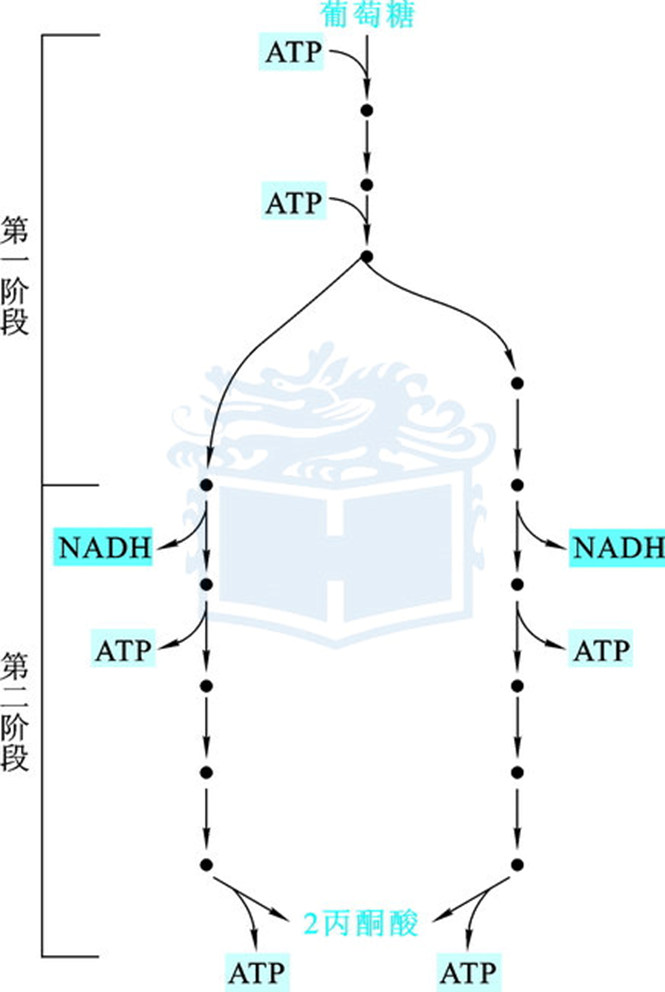
\includegraphics[width=0.4\linewidth]{Pics/糖酵解纵览}
	\caption{糖酵解纵览}
	\label{fig:糖酵解纵览}
\end{figure}

\begin{figure}[p]
	\centering
	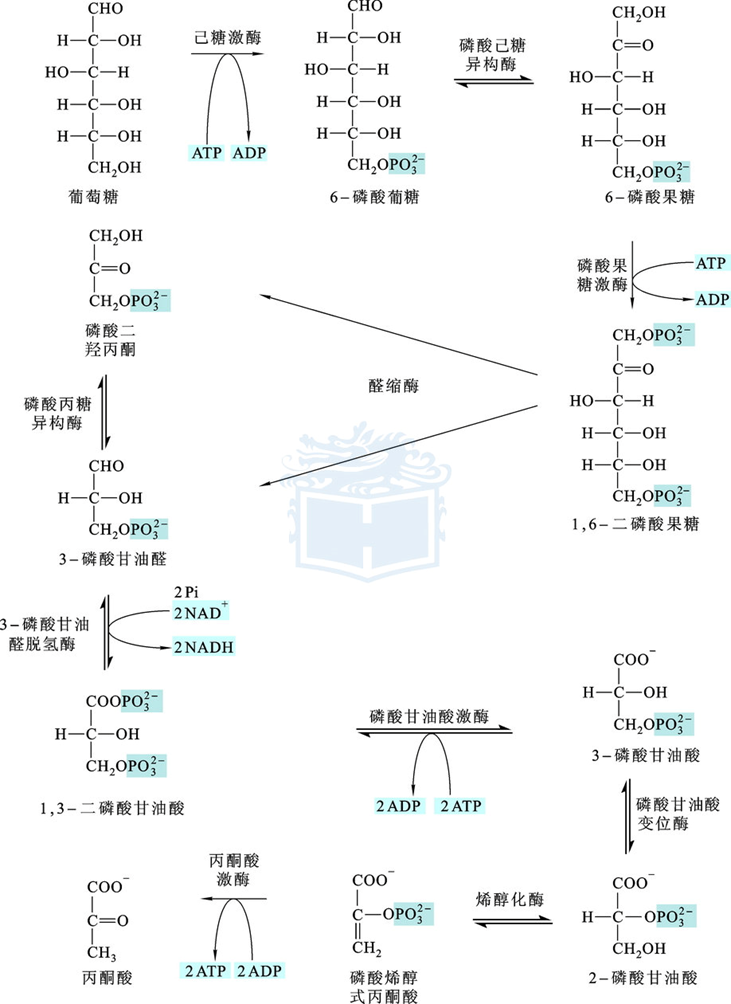
\includegraphics[width=\linewidth]{Pics/糖酵解的全部发硬}
	\caption{糖酵解的全部反应}
	\label{fig:all_reaction_glycolysis}
\end{figure}

下面分步介绍每步反应:

\subsubsection{葡萄糖的磷酸化}

\begin{center}
	葡萄糖+ATP$\xrightarrow[\text{己糖激酶或葡糖激酶}]{\ce{Mg^{2+}}}$6-磷酸葡糖+ADP
\end{center}

不可逆反应,由己糖激酶或葡糖激酶催化。己糖激酶利用诱导契合机制,避免ATP在活性中心的水解。

反应还需要\ce{Mg^{2+}},有时\ce{Mn^{2+}}可替代。细胞内所有涉及NTP或dNTP的反应都需要\ce{Mg^{2+}}。因为这些反应都依赖于一个亲核基团对磷酸基团P原子的亲核进攻。\ce{Mg^{2+}}和酶自带的碱性氨基酸残基可屏蔽解离状态的O原子所带的负电荷。如己糖激酶用K屏蔽$\gamma$-磷酸、用R屏蔽$\alpha$-磷酸的负电荷。

2-脱氧葡糖也可参与反应,生成2-脱氧-6-磷酸葡糖,是下一步异构反应的抑制剂。

葡萄糖磷酸化的意义:
\begin{itemize}
	\item 降低胞内葡萄糖浓度,有利于葡萄糖通过GLUT入胞;
	\item 提高葡萄糖的极性,避免葡萄糖离开细胞;
	\item 提高葡萄糖能量状态,使其不稳定。
\end{itemize}

己糖激酶和葡糖激酶的区别:(\autoref{tab:己糖激酶和葡糖激酶的区别})

\begin{table}[htbp]
	\centering
	\begin{tabularx}{\textwidth}{|c|C|C|}
		\hline
		特性 & 己糖激酶 & 葡糖激酶 \\ \hline
		存在 & 几乎所有的细胞 & 肝细胞、胰脏的$\upbeta$细胞 \\ \hline
		底物特异性 & 多数己糖 & 葡萄糖和 2-脱氧葡糖 \\ \hline
		对葡萄糖的$K_{m}$ & 低 & 高 \\ \hline
		$V_{max}$ & 低 & 高 \\ \hline
		产物反馈抑制 & G-6-P反馈抑制 & 不受G-6-P反馈抑制 \\ \hline
		基因表达 & 组成酶 & 诱导酶 \\ \hline
	\end{tabularx}
	\caption{己糖激酶和葡糖激酶的区别}
	\label{tab:己糖激酶和葡糖激酶的区别}
\end{table}

\begin{itemize}
	\item 己糖激酶是组成酶,与葡萄糖亲和力较高,能保证葡萄糖持续进入细胞;
	\item 葡糖激酶是诱导酶,与葡萄糖亲和力较低,血糖较高时才被诱导表达。
\end{itemize}

\subsubsection{6-磷酸葡糖的异构}

\begin{center}
	\ce{\text{6-磷酸葡糖} <=>[Mg^{2+}][\text{磷酸己糖异构酶}] \text{6-磷酸果糖}}
\end{center}

\subsection{NADH和丙酮酸的命运}

\subsubsection{有氧条件}

\paragraph{NADH}

有氧状态下,NADH将会把电子转移给呼吸链,产生更多ATP。
\begin{itemize}
	\item 在原核细胞,NADH很容易就可以到达呼吸链,因为呼吸链在细胞膜上;
	\item 在真核细胞,NADH要通过线粒体内膜就要经过专门的穿梭系统。
\end{itemize}

线粒体内膜上有3-磷酸甘油穿梭系统和苹果酸-天冬氨酸穿梭系统。脑细胞主要是前者, 肝细胞主要是后者。

\begin{description}
	\item[3-磷酸甘油穿梭系统] 如\autoref{fig:3-磷酸甘油穿梭系统},这种穿梭方式相当于把2个高能电子给了FAD,原本能产生2.5个ATP,现在只能产生1.5个。

	\begin{figure}[htbp]
		\centering
		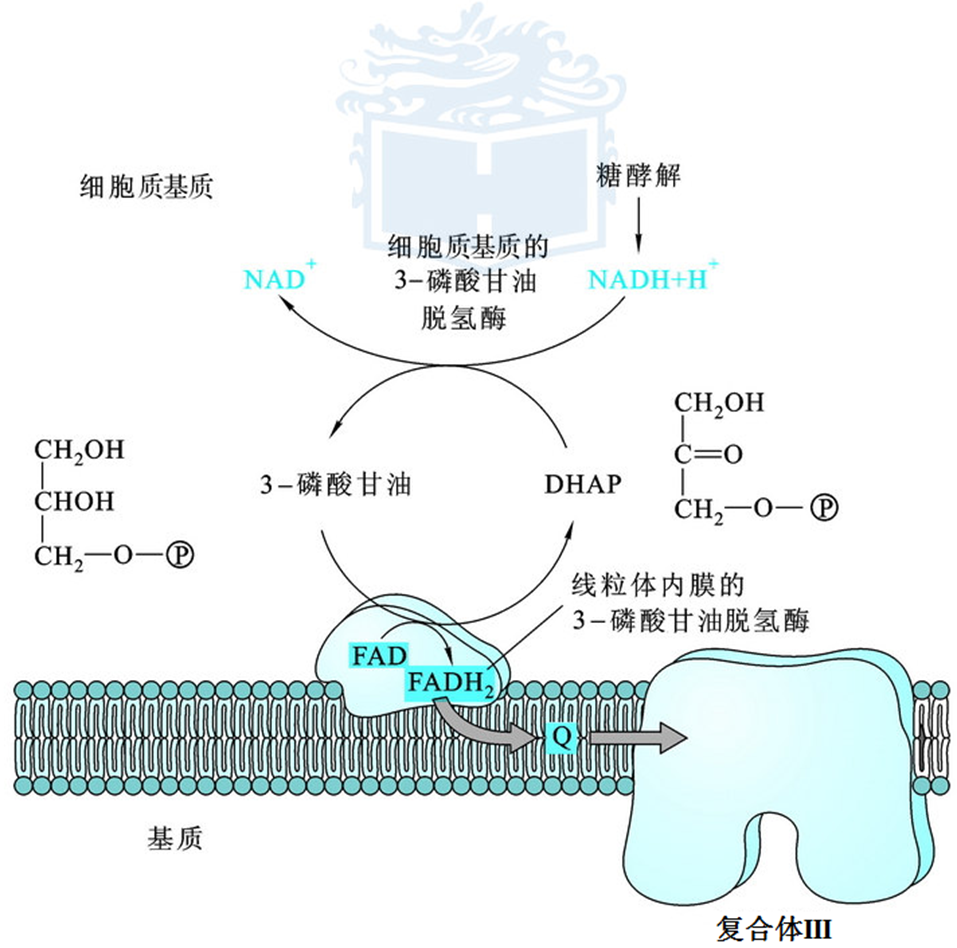
\includegraphics[width=0.7\linewidth]{Pics/3-磷酸甘油穿梭系统}
		\caption{3-磷酸甘油穿梭系统}
		\label{fig:3-磷酸甘油穿梭系统}
	\end{figure}

	\item[苹果酸-天冬氨酸穿梭系统] 如\autoref{fig:苹果酸-草酰乙酸穿梭系统},这一穿梭系统相当于用苹果酸把NADH的氢带进线粒体,最终可以无损耗地生成2.5个ATP。

	\begin{figure}[htbp]
		\centering
		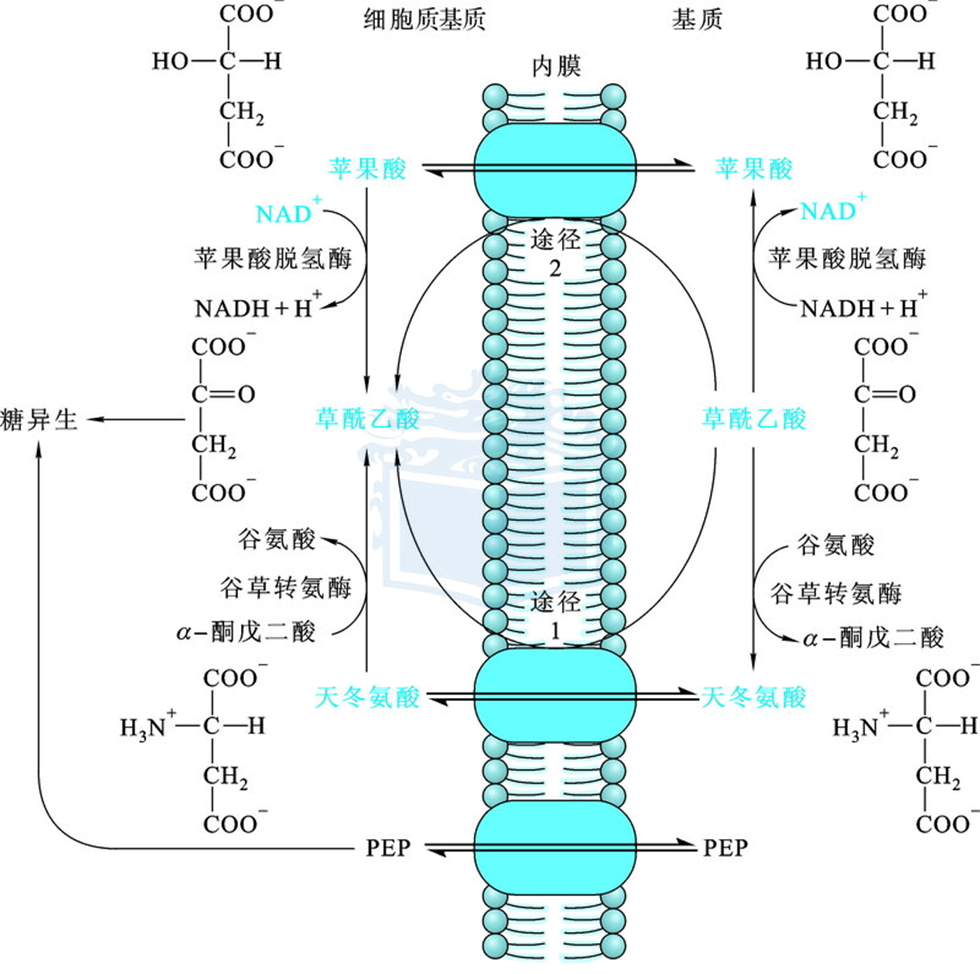
\includegraphics[width=0.9\linewidth]{Pics/苹果酸-草酰乙酸穿梭系统}
		\caption{苹果酸-草酰乙酸穿梭系统}
		\label{fig:苹果酸-草酰乙酸穿梭系统}
	\end{figure}

\end{description}

\paragraph{丙酮酸}

有氧条件下,丙酮酸将通过线粒体内膜上的丙酮酸转运蛋白,被线粒体基质内的丙酮酸脱氢酶系氧化成乙酰CoA。

\subparagraph{丙酮酸脱氢酶系的组成}

\begin{table}[htbp]
	\centering
	\begin{tabularx}{\textwidth}{|c|c|c|X|}
		\hline
		\textbf{酶} & \textbf{缩写} & \textbf{辅因子} & \multicolumn{1}{c|}{\textbf{催化反应}} \\ \hline
		丙酮酸脱氢酶 & E1 & TPP、Mg & 丙酮酸氧化脱羧 \\ \hline
		二氢硫辛酸转乙酰酶 & E2 & 硫辛酸、CoA & 氧化型硫辛酰胺的还原、羟乙基氧化为乙酰基、乙酰基的两次转移 \\ \hline
		二氢硫辛酸脱氢酶 & E3 & FAD、NAD$^{+}$ & 氧化型硫辛酰胺的再生 \\ \hline
	\end{tabularx}
	\caption{丙酮酸脱氢酶系的组成}
	\label{tab:丙酮酸脱氢酶系的组成}
\end{table}

丙酮酸脱氢酶系的反应如\autoref{fig:丙酮酸脱氢酶系}所示。

\begin{figure}[htbp]
	\centering
	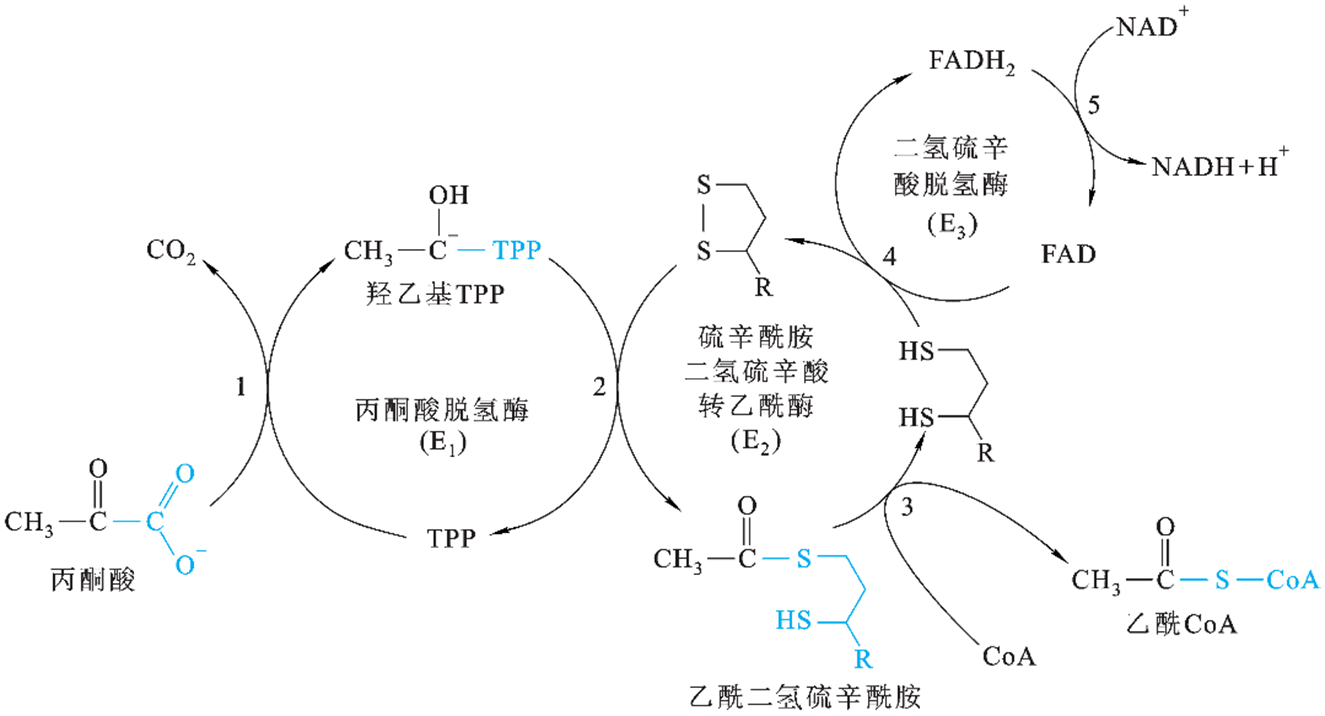
\includegraphics[width=\textwidth]{Pics/丙酮酸脱氢酶系}
	\caption{丙酮酸脱氢酶系}
	\label{fig:丙酮酸脱氢酶系}
\end{figure}

亚砷酸(砒霜的成分之一),能与还原型亚硫酰胺形成共价化合物(\autoref{fig:砒霜的毒性机理}),抑制整个丙酮酸脱氢酶系。它同样可抑制在三羧酸循环中的$\alpha$-酮戊二酸脱氢酶系中类似的反应。

\begin{figure}[htbp]
	\centering
	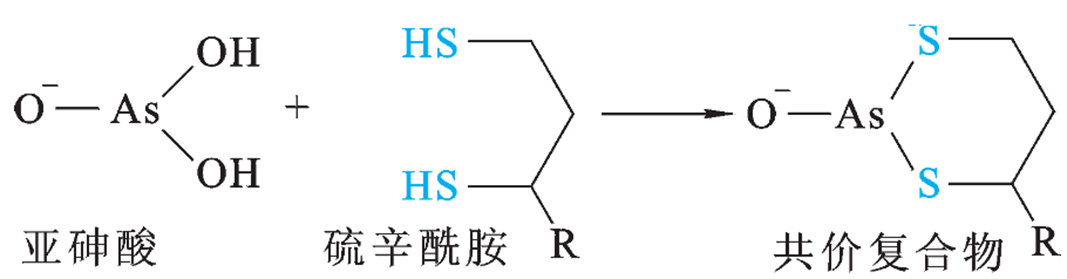
\includegraphics[width=0.5\linewidth]{Pics/砒霜有毒}
	\caption{砒霜的毒性机理}
	\label{fig:砒霜的毒性机理}
\end{figure}

\subsubsection{无氧条件}

无氧条件下,丙酮酸和NAD$^{+}$的命运是相互联系的。(\autoref{fig:丙酮酸的去路})不同生物使用的反应或许不同,但最终目的都是确保NADH变为NAD$^{+}$,即NAD$^{+}$再生。因为无氧条件下三羧酸循环不能进行。NADH不能消耗,最终将导致NAD$^{+}$耗尽,连糖酵解都无法进行。

\begin{figure}[htbp]
	\centering
	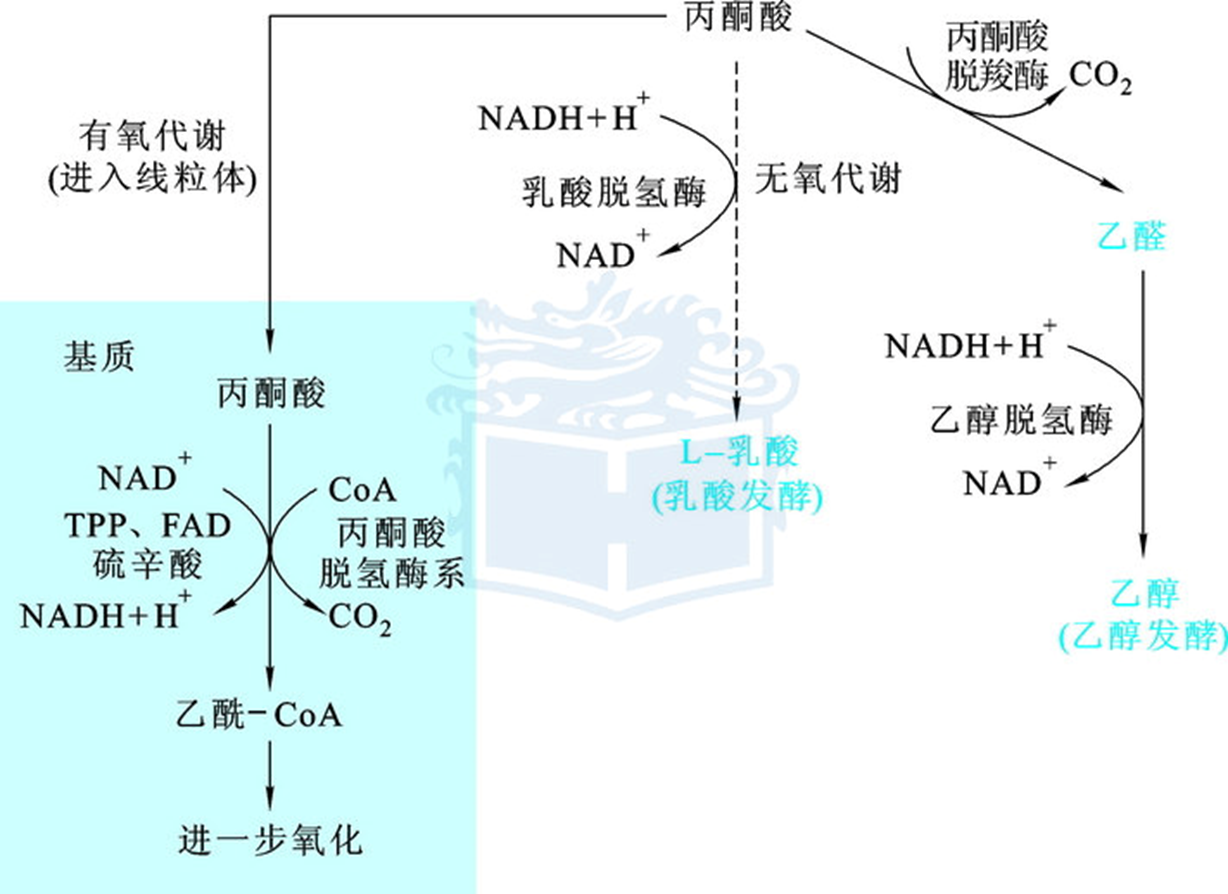
\includegraphics[width=0.7\linewidth]{Pics/丙酮酸的去路}
	\caption{丙酮酸的去路}
	\label{fig:丙酮酸的去路}
\end{figure}

\paragraph{乳酸发酵}

乳酸杆菌和其他一些微生物就是使用这条途径来完成NAD$^{+}$的再生。

高等动物的细胞在出现氧债的情况下,也会进行乳酸发酵,但是乳酸需要被运到肝细胞才能重新氧化成丙酮酸。哺乳动物红细胞无线粒体,故每时每刻都在进行乳酸发酵。

\paragraph{乙醇发酵}

许多微生物(如酿酒酵母)体内进行乙醇发酵。其中的丙酮酸脱羧酶依赖于TPP。

人体内虽然有乙醇脱氢酶,但是因为没有丙酮酸脱羧酶,故无法进行乙醇发酵。

\paragraph{其他形式的发酵}

有的微生物还可通过其他方式完成NAD$^{+}$的再生。无论是哪种形式的发酵,都是用NADH的电子去还原有机物罢了。

\begin{gs}[:不喝酒也醉酒的秘密]

	\hspace{2em}想象一下,吃碗面或薯片后竟然醉了!这不是玩笑,二战后,美国大兵查尔斯·斯瓦特就遇到了这种怪事。20年来,他没沾酒却总是醉醺醺的,肝脏也受尽折磨。直到1964年,他发现有个日本人和他同病相怜。25年后,医生终于诊断出他们得了“自动酿酒综合征”。原来,他们肠道里的酵母菌变异了,不断进行糖酵解和乙醇发酵。在医生建议下,斯瓦特服用了杀酵母的药物,直到1975年才恢复正常。

	\hspace{2em}医生诊断难,因为这种酵母菌本是肠道常客,谁会想到它能酿酒呢?至于变异原因,可能是广岛和长崎的核爆辐射导致的。
\end{gs}

\subsection{其他物质进入糖酵解}

\begin{figure}[htbp]
	\centering
	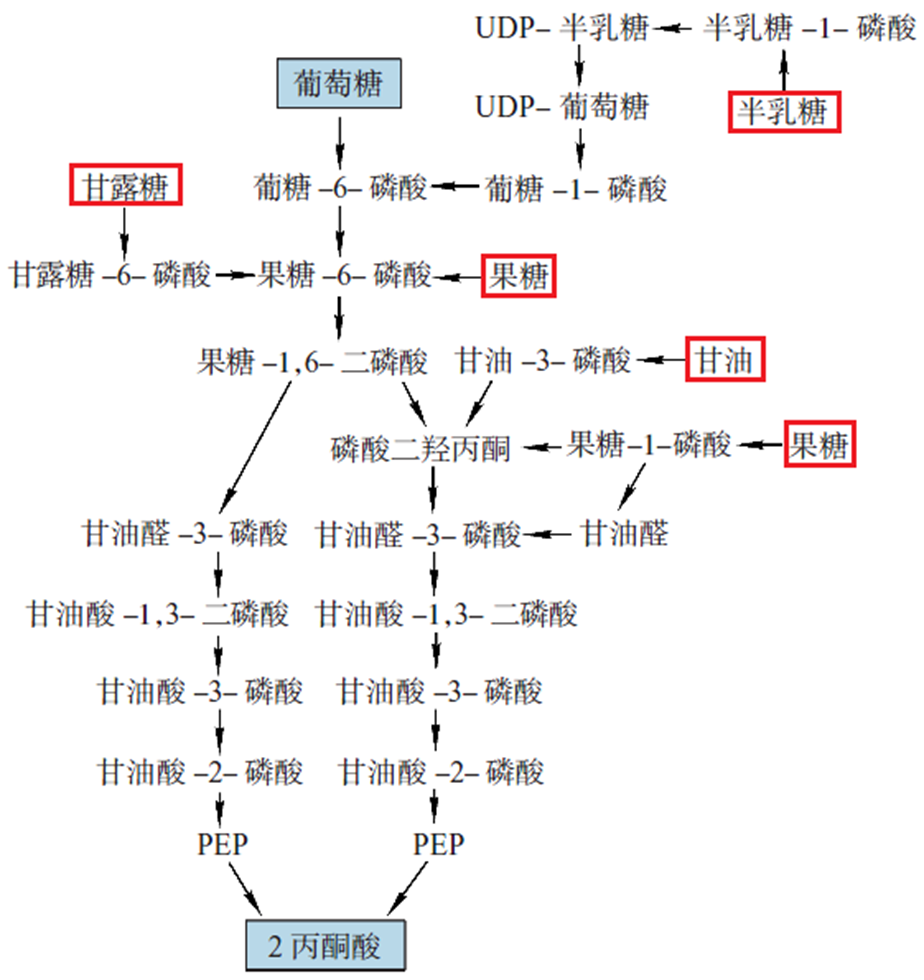
\includegraphics[width=0.8\linewidth]{Pics/其他物质进入糖酵解}
	\caption{其他物质进入糖酵解的途径}
	\label{fig:其他物质进入糖酵解的途径}
\end{figure}

\subsubsection{糖原}

糖原$\xrightarrow[\text{磷酸解}]{\text{糖原磷酸化酶a}}$1-磷酸葡萄糖$\xrightarrow{\text{磷酸葡糖变位酶}}$6-磷酸葡糖$\longrightarrow$糖酵解

\subsubsection{果糖}

果糖可通过两种方式进入糖酵解:
\begin{enumerate}
	\item (肌、肾)果糖$\xrightarrow{\text{己糖激酶}}$6-磷酸果糖$\longrightarrow$糖酵解
	\item (肝)果糖$\xrightarrow{\text{果糖激酶}}$1-磷酸果糖$\xrightarrow[\text{(醛缩酶B)}]{\text{1-磷酸果糖醛缩酶}}$磷酸二羟丙酮、D-甘油醛\\
	$\xrightarrow[\text{后者丙糖激酶}]{\text{前者TIM}}$3-磷酸甘油醛$\longrightarrow$糖酵解
\end{enumerate}

\subsubsection{甘露糖}

甘露糖$\xrightarrow{\text{己糖激酶}}$6-磷酸甘露糖$\xrightarrow{\text{磷酸甘露糖异构酶}}$6-磷酸果糖$\longrightarrow$糖酵解

\subsubsection{甘油}

甘油$\xrightarrow{\text{甘油激酶}}$3-磷酸甘油$\xrightarrow{\text{3-磷酸甘油脱氢酶}}$磷酸二羟丙酮$\xrightarrow{\text{磷酸丙糖异构酶}}$3-磷酸甘油醛$\longrightarrow$糖酵解

\subsubsection{半乳糖}

半乳糖进入糖酵解需要经过Leloir途径(\autoref{fig:leloir})。

\begin{figure}[htbp]
	\centering
	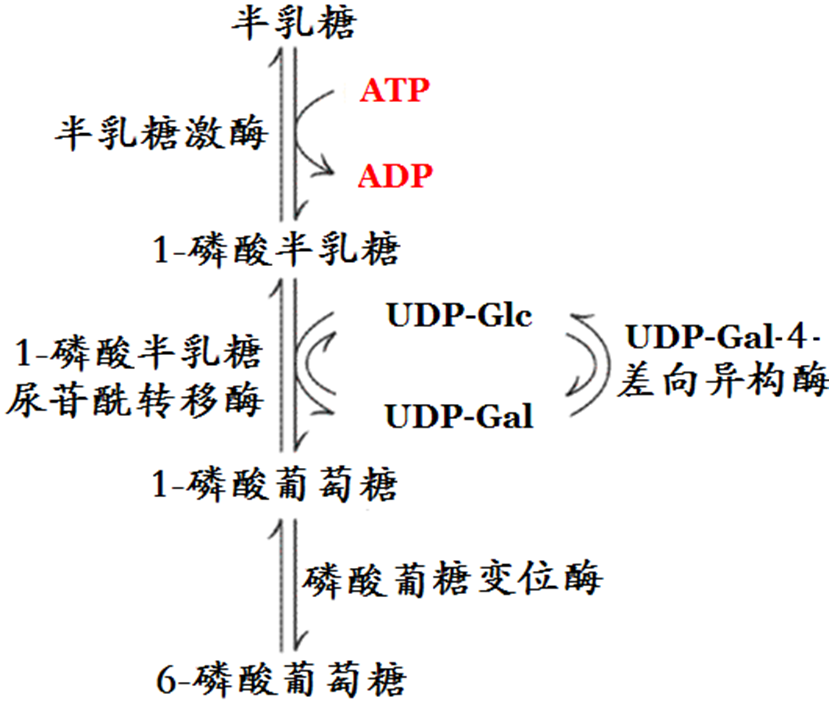
\includegraphics[width=0.4\linewidth]{Pics/Leloir途径}
	\caption{Leloir途径}
	\label{fig:leloir}
\end{figure}

\subsection{糖酵解的生理功能}

糖酵解较为普通的生理功能有:产ATP、为细胞内其他物质合成提供原料(\autoref{fig:糖酵解某些中间物的代谢流向})。下面介绍比较特别的功能。

\begin{figure}[htbp]
	\centering
	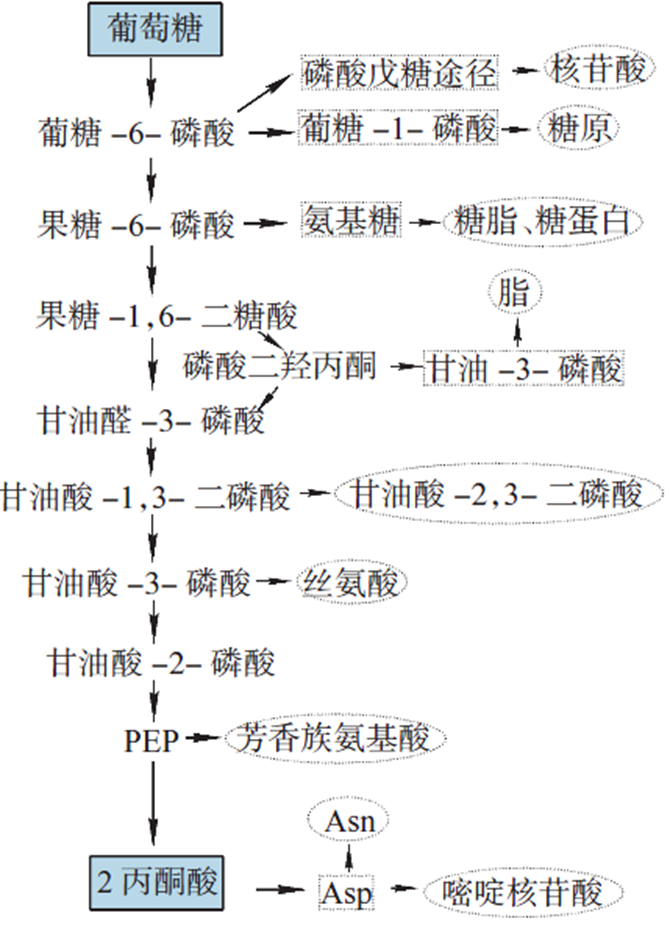
\includegraphics[width=0.4\linewidth]{Pics/糖酵解某些中间物的代谢流向}
	\caption{糖酵解某些中间物的代谢流向}
	\label{fig:糖酵解某些中间物的代谢流向}
\end{figure}

\subsubsection{癌细胞与糖酵解}

癌细胞生长速度很快,对能量需求高,常处于因血流不足而处在缺氧状态。受缺氧诱导,转录因子HIF-1$\upalpha$被激活,与DNA上缺氧应答元件结合,最后诱导参与糖酵解的酶和GLUT1、GLUT2的表达。

HIF-1$\upalpha$被激活的原理是:
\begin{itemize}
	\item 有氧条件下,该蛋白的一个Pro发生羟基化修饰,羟基的氧来源于氧气。这个羟基化使其容易被泛素化降解。
	\item 缺氧条件下,HIF-1$\upalpha$就可以稳定存在,作为转录因子诱导基因表达。
\end{itemize}

HIF-1$\upalpha$还可诱导血管内皮生长因子(VEGF)表达,促进新血管生长,为癌细胞供氧。

\subsubsection{糖酵解中一些酶的兼职功能}

\paragraph{磷酸己糖异构酶}

\begin{itemize}
	\item 兼职神经白介素;
	\item 作为自分泌运动因子。
\end{itemize}

\paragraph{3-磷酸甘油醛脱氢酶}

在细胞核中兼职尿嘧啶-DNA糖苷酶,参与DNA的碱基切除修复。

\paragraph{烯醇化酶}

\begin{itemize}
	\item 在细菌体内作为RNA降解体的一部分;
	\item 在真核生物体内,参与线粒体tRNA的运输;
	\item 在某些哺乳动物体内,作为细胞表面的受体结合纤维蛋白溶酶原和胞外基质,促进正常的细胞迁移;
	\item 病原体的烯醇化酶也有结合纤维蛋白溶酶原的活性,利用纤溶酶途径促进宿主组织的水解,有利于入侵;
\end{itemize}

\paragraph{醛缩酶}

\begin{itemize}
	\item 作为胞内葡萄糖水平高低的感应器,帮助细胞实时探测葡萄糖水平。
	\item 通过改变AMP激活的蛋白激酶(AMPK)的活性对细胞内葡萄糖水平的变化及时作出反应:促进多种蛋白质(如regulator、V型ATP酶、轴蛋白和肝激酶B1(LKB1)等)聚合在一起,最终激活依赖溶酶体的AMPK途径,进而激活AMPK。AMPK可催化胞内多种限速酶的磷酸化修饰,导致多条合成代谢途径的关闭。
\end{itemize}

\subsection{糖酵解的调节}

